% displayname : Modèle scalaire de la lumière
\documentclass[12pt,fancy]{cours}
\Chapit{3}{1}
\begin{document}
\maketitre{
En première année, vous avez étudié les phénomènes optiques en décrivant la lumière par un ensemble de rayons lumineux indépendants. Cette approche, appelé optique géométrique, n'explique pas les phénomènes d'interférence et de diffraction, qui proviennent du caractère ondulatoire de la lumière. Dans ce chapitre, nous posons les bases de l'optique ondulatoire, en décrivant la lumière par une vibration lumineuse scalaire. Cette théorie reste une approximation de la réalité, puisque l'on néglige le caractère vectoriel des ondes électromagnétiques, et donc les effets de polarisation.
}
{
\item Cours Optique 1 et 2 - 0, Signaux 1 - 0
\item Document de cours Optique 1 - 1, 2 - 1 à 3
\item TD Optique 1 et 2, Signaux 1
}


%%%%%%%%%%%%%%%%%%%%%%%%%%%%%%%%%%%%%%%%%%%%%%%%%%%%%%%%%%%%%%%%%%%%%%%%%%
\section{Le modèle scalaire de la lumière}
\label{sec:modele}
\subsection{Cadre de l’optique géométrique}

\parag{Généralités sur la lumière}

Une onde est constituée par une perturbation qui se propage de proche en proche, avec transport d'énergie et sans qu'il y ait un transport de matière. Maxwell a montré, en 1876, que la lumière était constituée par la propagation d'un champ électromagnétique $(\vec{E}, \vec{B})$ : on parle d'onde électromagnétique. Comme toute onde, la lumière peut se décomposer en une superposition d'ondes sinusoïdales, dites \imp{monochromatiques} (\guill{d'une seule couleur}). Ses caractéristiques sont les suivantes.
\begin{liste}
  \item \udl{Domaine temporel} :
  % \element[:]{Domaine temporel}
  période $T$ (en \SI{}{s}), fréquence $\nu=\frac{1}{T}$ (en \SI{}{Hz}), et pulsation $\omega = 2\pi \nu$ (en \SI{}{rad.s^{-1}});

  \item \udl{Domaine spatial} :
  % \element[:]{Domaine spatial}
  longueur d'onde $\lambda$ (en \SI{}{nm}), nombre d'onde $\sigma=\frac{1}{\lambda}$ (en \SI{}{m^{-1}}), et norme du vecteur d'onde $k=2\pi \sigma$ (en \SI{}{rad.m^{-1}}).

\end{liste}

\begin{figure}[H]
  \centering
  \subfigure[]{\label{fig:}
  
\includegraphics{wave_t.pdf}
  }\hspace{1cm}
  \subfigure[]{\label{fig:}
  
\includegraphics{wave.pdf}
  }
  \caption{}
  \label{fig:}
\end{figure}
Certaines propriétés de la lumière dépendent du milieu dans lequel elle se propage. Nous considérerons ici soit le vide, soit un milieu transparent, homogène et isotrope (THI).
\begin{liste}
  \item \udl{Vide}
  % \element[.]{Vide}
  
  On note $\lambda_0$ la longueur d'onde dans le vide. La fréquence $\nu$ et la longueur d'onde $\lambda_0$ ne sont pas indépendants : ces grandeurs sont liées par une \imp{relation de dispersion}.
  \begin{prop}[Relation de dispersion dans le vide]\label{prop:}
    La \imp{relation de dispersion} de la lumière dans le \imp{vide} est donnée par
    $$ 
    \lambda_0 = \frac{c}{\nu},
    $$
    où $c\simeq\SI{3.0e8}{m.s^{-1}}$ est la célérité de la lumière dans le vide.
  \end{prop}

Les différents domaines du spectre électromagnétique sont représentés sur la \Fig{spectre} en fonction de la fréquence $\nu$ et de la longueur d'onde dans le vide correspondante $\lambda_0$.

  \item \udl{Milieu transparent homogène isotrope (THI)}
  
  Un milieu est THI lorsqu'il est
  
  \begin{enumerate}
    \item transparent : il n'absorbe pas la lumière ;
    \item homogène : ses propriétés optiques sont les mêmes en tout point ;
    \item isotrope : ses propriétés optiques sont les mêmes dans toutes les directions.
  \end{enumerate}
  Les milieux THI incluent les milieux diélectriques peu absorbant (l'air, l'eau, le verre), mais excluent les milieux conducteurs électriques, ou magnétiques.
  Un milieu THI
  est caractérisé par un coefficient sans dimension \fbox{$n >1$}, appelé \imp{indice de réfraction}, tel que la vitesse $v$ de la lumière dans le milieu vérifie
  % \begin{equation}
  \eqbox[]{
    v = \frac{c}{n} < c.
    }
    L'indice de réfraction $n$ est réel (milieu transparent), indépendant de la position (milieu homogène), et indépendant de la direction de l'onde (milieu isotrope).
    La relation de dispersion dans un milieu THI est donc  $\lambda = \frac{v}{\nu} = \frac{v}{c} \cdot \frac{c}{\nu} = \frac{\lambda_0}{n}$, où $\lambda_0$ est la longueur d'onde dans le vide.
    \begin{prop}[Relation de dispersion dans un milieu THI]\label{prop:}
      La \imp{longueur d'onde} $\lambda$ dans un milieu THI est reliée à la longueur d'onde dans le vide $\lambda_0$ par
      $$
      \lambda = \frac{\lambda_0}{n}.
      $$
    \end{prop}
  \end{liste}

\begin{exemple}{Milieu THI}
  Calculer la vitesse $v$  et la longueur d'onde $\lambda$ des ondes lumineuses dans les milieux suivants.
  \begin{quest}
    \item	Dans l'air, d'indice de réfraction $n\simeq 1$, à la fréquence $\nu = \SI{5.0e14}{Hz}$.
    \item Dans l'eau, d'indice de réfraction $n\simeq \num{1.33}$, à la fréquence $\nu = \SI{6.0e14}{Hz}$.
    \item Dans le verre \emph{crown}, d'indice de réfraction  $n\simeq \num{1.5}$, à la fréquence $\nu = \SI{7.0e14}{Hz}$.
    \item Dans le verre \emph{flint}, d'indice de réfraction  $n \simeq \num{1.7}$, à la fréquence $\nu = \SI{8.0e14}{Hz}$.
  \end{quest}
\end{exemple}
\examplesol{}

L'indice de réfraction dépend aussi de la longueur d'onde $\lambda$. Pour une onde de fréquence $\nu$ donnée, la longueur d'onde dans le milieu $\lambda$ est plus courte que celle dans le vide $\lambda_0$. Elle vérifie $\lambda_0 = n \lambda$.

%%%%%%%%%%%%%%%%%%%%%%%%%%%%%%%%
\begin{figure}[H]
\centering
\subfigure[]{\label{fig:}

\includegraphics[width=\textwidth]{Domaines_du_spectre_EM.pdf}
}
\subfigure[]{\label{fig:}

\includegraphics[width=0.7\textwidth]{visible_spectrum.jpg}
}
\caption{(a) Domaines du spectre électromagnétique (au-dessus) et  (b) agrandissement correspondant au domaine visible (en dessous). Les micro-ondes se situent entre l'infrarouge et les ondes radio. \Wiki}
\label{fig:spectre}
\end{figure}
%%%%%%%%%%%%%%%%%%%%%%%%%%%%%%%%%%

%\subsection{Pinceau lumineux (optique géométrique)}
\parag{Cadre de l'optique géométrique}
Il s'agit du modèle de la lumière que vous avez étudié en PCSI.
% Dans le cadre de l'optique géométrique étudié en $1^{\rm ere}$ année, tous les phénomènes ondulatoires ont

\begin{prop}[Cadre de l'optique géométrique]\label{prop:}
  L'optique géométrique suppose qu'un faisceau lumineux est constitué de \imp{rayons lumineux} :
  \begin{enumerate}
    \item \imp{indépendants} ;
    \item \imp{rectilignes} dans un milieu THI.
  \end{enumerate}
\end{prop}
 Un rayon lumineux n'a pas d'existence physique, mais est un outil théorique utile pour décrire la formation des images.
%Dans un milieu homogène, transparent et isotrope ces rayons sont des lignes droites.
Cette description de la lumière ne prend pas en compte les phénomènes ondulatoires, à savoir la diffraction et l'interférence. 
% Pour cette raison, elle est valable lorsque :
\begin{enumerate}

\item Les rayons lumineux sont \imp{indépendants} si l'on peut négliger les \imp{interférences}.

Les conditions d'interférences seront étudiées dans le \refChap{3}{2}.

% La lumière ne vérifie pas les conditions d'interférence ou de cohérence spatiale ou temporelle, dont nous reparlerons.
% la largeur spectrale en fréquence de la lumière $\Delta \nu$ est grande devant la fréquence de détection $\nu_r$ du récepteur de lumière, soit
% \eqbox[]{
% \Delta \nu \gg \nu_r.
% }
%  Cette propriété assure l'\imp{indépendance} des rayons et permet de négliger les \imp{interférences}.


  % Elle est vérifiée pour de la lumière blanche, par exemple produite par une lampe ou le Soleil observée à l'œil nu mais pas pour de la lumière laser. On peut donc observer une figure de diffraction si l'on éclaire une fente fine avec un laser. Nous discuterons de cette condition dans le \Chap{}.

  \item Les rayons lumineux sont \imp{rectilignes} si l'on peut négliger la \imp{diffraction}. 


La taille caractéristique $a$ des diaphragmes et obstacles rencontrés par les rayons lumineux est grande devant la longueur d'onde caractéristique de la lumière $\lambda$. L'angle typique de diffraction vaut $\theta_{\rm diff} = \frac{\lambda}{a}$. Si $\theta$ est l'angle apparent typique sous lequel sont vus les dispositifs optiques, alors on doit avoir
\eqbox[]{
\theta_{\rm diff}  = \frac{\lambda}{a} \ll \theta.
}
Cette propriété assure la propagation des rayons en \imp{ligne droite} au voisinage d'un obstacle, et permet de négliger la \imp{diffraction} ;

 % La lumière visible est de longueur d'onde moyenne $\lambda \simeq \SI{550}{nm}$ dans le vide ; des obstacles de taille supérieure à $L \simeq \SI{1}{mm}$ satisfont donc à cette condition.

\end{enumerate}


 \begin{exemple}{Validité de l'optique géométrique}
  
% \begin{quest}
  % \item
  Un faisceau laser, de longueur d'onde  $\lambda_0=\SI{632}{nm}$, se propage dans le vide, et traverse un diaphragme circulaire de rayon $a=\SI{1}{mm}$ avant de  frapper un récepteur de lumière dont les pixels sont de largeur $d=\SI{100}{\mu m}$. Le récepteur est situé à une distance $D=\SI{2}{m}$ du diaphragme. 
  
  Le cadre de l'optique géométrique est-il valide dans cette situation ?
  % \item  Un expérimentateur, dont les yeux ont un temps de réponse $\tau_r \sim \SI{0.1}{s}$, observe un point d'un écran impacté par plusieurs rayons provenant d'une source de lumière blanche de largeur spectrale $\Delta \nu \sim \SI{e14}{Hz}$. Même question si on remplace la source de lumière blanche par un laser, dont la largeur spectrale vaut $\Delta \nu = \SI{50}{kHz}$.
% \end{quest}
 \end{exemple}
 \examplesol{
 % \begin{quest}
   % \item
   On trouve un angle apparent de résolution $\theta \simeq \frac{d}{D} = \SI{5e-5}{}$, et donc $\frac{\lambda_0}{\theta} \sim \SI{e-2}{m}$, qui est plus grand que $a=\SI{e-3}{m}$. La diffraction est donc importante dans cette expérience.
   % \item On trouve une fréquence de détection $\nu_r = \frac{1}{\tau_r} \sim \SI{10}{Hz}$.
 % \end{quest}
 }

% Typiquement pour des obstacles de l'ordre du millimètre et de la lumière visible, cette condition est bien vérifiée. Dans le cas contraire, le caractère ondulatoire de la lumière devient important (diffraction, interférences).



%
% La lumière visible, de largeur spectrale en longueur d'onde $\Delta \lambda \simeq \SI{300}{nm}$, ne représente qu'une petit partie des ondes électromagnétiques  Le spectre des ondes électromagnétiques dans le vide est présenté sur la \Fig{spectre}. La longueur d'onde $\lambda$ correspond à la distance parcourue par une onde monochromatique pendant une période ; nous la noterons $\lambda_0$ quand l'onde se propage dans le vide. Une onde lumineuse est aussi caractérisée par sa fréquence~$\nu$, qui vérifie
% \begin{equation}
% \lambda_0 = \frac{c}{\nu}.
% \end{equation}
% Plus une onde a une fréquence élevée ou une longueur d'onde petite, plus elle est énergétique.
% %En général, la lumière visible est une superposition d'onde monochromatiques. Pour une source thermique comme le Soleil ou certaines lampes à vapeur, on parle de lumière blanche (addition de toutes les couleurs).


%À l'interface de séparation entre deux milieux (dioptre), les rayons obéissent aux lois de Snell-Descartes rappelées en Sec.~\ref{sec:snell_descartes}.
%: les rayons incidents réfléchis et réfractés appartiennent au plan d'incidence (qui inclut la normale au dioptre et le rayon incident) et $n_1\sin(i_1)=n_2\sin(i_2)$; pour la réflexion $i=-r$ (opposés par rapport à la normale).

% en bonne approximation selon la loi de Cauchy
%\begin{equation}
%n(\lambda)=A+\frac{B}{\lambda^2}
%\end{equation}
%où $A$ et $B$ sont deux constantes qui dépendent du matériau. On dit que le milieu est \important{dispersif}, car il peut disperser les composantes d'un lumière polychromatique en se différentes composantes monochromatiques. Pour éviter cette difficulté liée à la dispersion d'un milieu, on considère généralement des lumières monochromatiques (en particulier celles émises par des lasers qui le sont en très bonne approximation).
%On dit d'un milieu qu'il est plus \important{réfringent} qu'un autre s'il possède un indice plus élevé.


%\subsection{Onde (optique ondulatoire) ou particule (mécanique quantique)?}
%Une description plus réaliste de la lumière est celle d'un champ électromagnétique contenant de l'énergie, qui se propage dans toutes les directions qui lui sont offertes. Mais au niveau microscopique, ce champ électromagnétique est constitué de photons, qui sont des particules de masse nulle. Les photons sont créés lors d'un processus d'émission, où un atome excité (par exemple thermiquement) d'énergie $E_2>E_1$ relaxe très rapidement vers un niveau d'énergie inférieur $E_1$ en émettant un photon de fréquence
%\begin{equation}
%\nu=\frac{E_2-E_1}{h}
%\end{equation}
%où $h\simeq \SI{6.6e-34}{J.s}$ est la constante de Planck. Ces valeurs d'énergies autorisées discrètes (quantifiées) s'expliquent dans le cadre de la mécanique quantique, et une description rigoureuse de la lumière nécessite un cadre complètement quantique.
%
%La fréquence $\nu$ correspond aussi à la fréquence de l'onde lumineuse, qui si elle est unique est qualifiée de monochromatique. Dans le domaine visible, il est courant de caractériser l'onde plutôt par sa longueur d'onde telle que
%\begin{equation}
%\lambda=\frac{c}{\nu}=cT
%\end{equation}
%qui correspond donc à la distance parcourue par une onde monochromatique durant une période $T$. On notera donc que plus une onde a une fréquence élevée (ou une longueur d'onde petite), plus elle est énergétique.
%En général, la lumière visible est une superposition d'onde monochromatiques. Pour une source thermique comme le Soleil ou certaines lampes à vapeur, on parle de lumière blanche (addition de toutes les couleurs).



%\subsection{L'indice optique}
%Dans un milieu transparent (c'est-à-dire qui laisse passer la lumière sans l'absorber ou la réfléchir en totalité, par exemple l'eau, le verre ou l'air) la lumière se propage à la vitesse $v<c$ et on note $v=c/n$ où $n$ désigne l'indice optique du milieu. Il dépend tout d'abord de la nature du milieu. Pour l'air en excellente approximation $n\simeq 1$, pour l'eau $n\simeq 1.33$ et pour le verre en général $n\simeq 1.5$. L'indice dépend aussi de la longueur d'onde, en bonne approximation selon la loi de Cauchy
%\begin{equation}
%n(\lambda)=A+\frac{B}{\lambda^2}
%\end{equation}
%où $A$ et $B$ sont deux constantes qui dépendent du matériau.
%On dit d'un milieu qu'il est plus \important{réfringent} qu'un autre s'il possède un indice plus élevé.

\subsection{Cadre de l’optique scalaire}

Nous souhaitons sortir du cadre de l’optique géométrique pour expliquer les phénomènes de diffraction et d’interférence. Nous savons que la lumière est décrite par des champs électrique $\Vec{E}$ et magnétique $\Vec{B}$.
Dans un milieu \imp{homogène isotrope}, les composantes cartésiennes de ces champs ($E_x$, $E_y$, etc.) obéissent toutes à la même équation de propagation (l'équation de Helmholtz, que nous verrons en électromagnétisme). Il est donc possible de représenter l'onde lumineuse par une seule composante du champ électrique, qui est une fonction \imp{scalaire} de la position $M$ et du temps $t$, appelée \imp{vibration lumineuse} et notée $\vib(M,t)$.

%\noindent La vibration lumineuse obéit à la même équation de propagation, et donc possède la même phase que les composantes de $\vv{E}$ et $\vv{B}$. Son amplitude est reliée à l'intensité de l'onde électromagnétique.
\begin{remarque}
  Le modèle scalaire de la lumière rend bien compte des observations
  %(en particulier en ce qui concerne le calcul de l'intensité lumineuse)
   lorsque les ondes sont non polarisées, ou bien sont toutes polarisées de la même façon.
  En revanche, le modèle scalaire ne permet pas d'interpréter l'absence d'interférences pour des polarisations orthogonales ou la propagation de la lumière dans les milieux anisotropes.

\end{remarque}

Dans le cadre de l'optique scalaire, nous pouvons conserver la notion de \imp{rayon lumineux} et supposer que la lumière emprunte le chemin défini par l'optique géométrique, et que la vibration lumineuse $\vib(M,t)$ se propage le long des rayons lumineux. Par contre, contrairement au cadre de l'optique géométrique, les rayons lumineux ne se propagent pas forcément en ligne droite dans un milieu homogène isotrope, et ne sont pas forcément indépendants.

\begin{prop}[Cadre de l'optique scalaire]\label{prop:vibration}
Dans le cadre de l'optique scalaire, on décrit l'onde lumineuse par une composante quelconque du champ électrique, que l'on appelle \important{vibration lumineuse} et notée $\vib(M,t)$. La vibration lumineuse se propage le long des \imp{rayons lumineux} de l'optique géométrique, qui ne sont 
\begin{enumerate}
  \item ni \imp{rectilignes} en général (diffraction) ;
  \item ni \imp{indépendants} en général (interférences).
\end{enumerate}
\end{prop}
En pratique, les rayons lumineux sont toujours rectilignes dans un milieu homogène isotrope, sauf au voisinage d'un obstacle (diaphragme, bord d'une lentille, etc), auquel cas un phénomène de diffraction a lieu.
Dans le cas important d'une lumière \imp{monochromatique}, la vibration lumineuse est sinusoïdale :
\eqbox[]{
\label{eq:expression_vib}
   \vib(M,t) = A(M)\cos\left(\omega t-\varphi({M})\right).
}
Le coefficient $A(M)$, qui dépend du point $M$, est l'amplitude de l'onde lumineuse, tandis que $\vphi(M)$ est la phase à l'origine de l'onde en $M$. Nous souhaitons à présent comprendre comment se propage la vibration lumineuse, autrement dit comment trouver la vibration lumineuse en un point $M$ connaissant celle en un autre point $S$.


%où $0<\alpha\leq 1$ est un coefficient d'atténuation de l'amplitude de l'onde lumineuse lors de sa propagation. Nous avons aussi identifié la phase au point $M$ comme étant $\vphi(M)=\varphi_S+\omega\tau_{SM}$.
%\begin{remarque}
%On peut généraliser le résultat précédent entre deux points quelconques $M$ et $N$ pour écrire que le déphasage entre deux points quelconques est de la forme
%\begin{equation}
%\vphi(M)-\varphi_N=\omega\tau_{NM}.
%\end{equation}
%\end{remarque}
%L'objectif de la suite est d'obtenir une expression explicite du retard $\tau_{SM}$ afin de parvenir à exprimer le déphasage de l'onde au cours de sa propagation.



\subsection{Chemin optique et phase}

\parag{Chemin optique}
Considérons la propagation d'un rayon lumineux d'un point $S$ à un point $M$.
%  et notons $\tau_{SM}$ le temps de parcours de l'onde lumineuse du point $S$ au point $M$.

\begin{definition}[Chemin optique]\label{def:chemin}
  Soit $\tau_{SM}$ le \imp{temps de parcours} de l'onde lumineuse du point $S$ au point $M$.
On appelle \important{chemin optique} de $S$ à $M$ la grandeur, homogène à une distance,
    \begin{equation*}
    \opt{SM}=c\,\tau_{SM}.
    \end{equation*}
  \end{definition}
\noindent Le chemin optique a les propriétés suivantes.

\begin{liste}
  \item \udl{Milieu THI}
  
  Soit $SM$ le chemin géométrique (la distance) parcouru par le rayon entre $\rm S$ et $\rm M$. Dans un milieu THI d'indice de réfraction $n$, le chemin optique a pour expression
  \eqbox[]{
    \opt{SM} = n SM.
    }
    \begin{preuve}
      Lorsque le milieu est homogène isotrope, d'indice de réfraction $n$, le temps de parcours vaut $\tau_{SM} =  \frac{SM}{v} =  n \frac{SM}{c}$, et donc le chemin optique s'écrit bien $\opt{SM} = n SM$.
    \end{preuve}
    
    \item \udl{Additivité} 
    
    Pour tout point intermédiaire $\rm P$ le long du rayon lumineux allant de $\rm S$ à $\rm M$, on a (voir \Fig{chemin})
    \eqbox[]{
      \opt{SM} = \opt{SP} + \opt{PM}.
      }
    \end{liste}



\begin{figure}[H]
\centering
\subfigure[]{\label{fig:chemin}

\includegraphics[scale=1]{chemin.pdf}
}\hspace{1cm}
\subfigure[]{\label{fig:malus}

\includegraphics[scale=1]{Malus.pdf}
}
\caption{(a) Une onde lumineuse se propage d'un point $S$ à un point $M$ en passant par un point $P$ en un temps $\tau_{SM}$. Le chemin optique entre $S$ et $M$ est défini par $\opt{SM} = c \tau_{SM}$. Le chemin optique est additif : $\opt{SM} = \opt{SP} + \opt{PM}$. (b) Théorème de Malus : les rayons lumineux sont orthogonaux aux surfaces d'onde, d'équation $\vphi(M) = \cte$.}
\end{figure}


%Notons $s(P)$ l'abscisse curviligne du point $P$ le long du rayon lumineux entre le point source $S$ et le point d'observation $M$. Par définition, la vitesse de la vibration lumineuse en $P$ est donnée par $\frac{\d s(P)}{\d t} = c(P)=\frac{c}{n(P)}$ et donc
%\begin{equation}
%\tau_{SM}=\int_{0}^{\tau_{SM}}\d t=\int_{S}^{M}\frac{\d t}{\d s}\d s=\frac{1}{c}\int_{S}^{M}n(P)\,\d s
%\end{equation}

   % À la constante $c$ près (vitesse de la lumière dans le vide), le chemin optique indique donc le temps de parcours entre la source et le point d'observation.
\parag{Lien avec la phase}
 Le chemin optique permet d'exprimer simplement le \imp{déphasage}, ou retard de phase, $\vphi(M) - \vphi(S)$ subit par l'onde lors de sa propagation entre les points $\rm S$ et $\rm M$, dans le cas d'une vibration lumineuse monochromatique. En effet, la vibration lumineuse met un temps $\tau_{SM}$ pour se propager le long du rayon lumineux :
les fonctions $
s(S,t)$ et $s(M,t+\tau_{SM})$ ont donc la même phase. On trouve donc,
\begin{equation}
  \omega t - \vphi(S) =\,\omega t + \omega \tau_{SM} - \vphi(M), \forall t,
\end{equation}
soit
    \begin{equation}
    \label{eq:dephasage_source_point_M}
    \vphi(M)-\vphi(S) = \omega \tau_{SM} = \frac{\omega}{c}\opt{SM}=\frac{2\pi}{\lambda_0}\opt{SM},
    \end{equation}
d'après la relation de dispersion de la lumière dans le vide.
    \begin{theorem}[Formule du déphasage]\label{form:}
      Les phases en deux points $\rm S$ et $\rm M$ d'un \imp{même rayon lumineux} sont reliées par
      $$
      \vphi(M) - \vphi(S) =  \frac{2\pi}{\lambda_0}\opt{SM}.
      $$
    \end{theorem}

\begin{remarque}
Il existe une exception à l'\Eq{dephasage_source_point_M} dans deux situations. Une réflexion sur
\begin{enumerate}
  \item une surface métallique ;
  \item ou un milieu plus réfringent (réflexion sur le verre dans l'air par exemple);
\end{enumerate}
s'accompagne d'un déphasage de $\pi$, de sorte que
   \begin{equation}
   \vphi(M)-\vphi(S)=\frac{2\pi}{\lambda_0}\opt{SM}+\pi.
   \end{equation}
% sur une surface métallique ou bien qu'elle subit une réflexion sur un milieu plus réfringent (réflexion air$\,\rightarrow\,$verre par exemple), 
% alors il faut rajouter « à la main » un déphasage supplémentaire de $\pi$, de sorte que
%    \begin{equation}
%    \vphi(M)-\vphi(S)=\frac{2\pi}{\lambda_0}\opt{SM}+\pi.
%    \end{equation}
\end{remarque}

%
%    \parag{Surface d'onde}
%
%

    \parag{Surface d'onde} La fonction $\vphi(M)$ est une fonction de la position $M$ dans l'espace. Les points $M$ tels que $\vphi(M) = \cte$ sont les points de même phase de l'onde lumineuse. Ils forment une surface dans l'espace, appelée \imp{surface d'onde}.

\begin{definition}[Surface d'onde]\label{def:}
On appelle \imp{surface d'onde} d’une vibration lumineuse monochromatique le lieu des points $M$ tel que
\begin{equation*}
\vphi(M) =\cte.
\end{equation*}

\end{definition}
% \noindent Supposons que l’onde lumineuse soit produite par une source ponctuelle $S$. D’après l’\Eq{dephasage_source_point_M}, une surface équiphase vérifie $\opt{SM}=\cte$ : sur une surface d'onde, le chemin optique est constant.
\noindent
Ainsi, deux points $\rm S$ et $\rm M$ appartenant à une même surface d’onde ont même phase $\vphi(S) = \vphi(M)$. Nous avons donc deux concepts pour décrire la lumière issu de deux approches différentes :
\begin{enumerate}
  \item le rayon lumineux, issu de l'optique géométrique ;
  \item la surface d'onde, issu de l'optique ondulatoire.
\end{enumerate}
Ces deux notions sont reliés par un théorème, appelé \imp{théorème de Malus}, voir \Fig{malus}.
\begin{prop}[Théorème de Malus]\label{form:malus}
Dans un milieu THI, les rayons lumineux sont en tout point \imp{orthogonaux} aux surfaces d'onde.
\end{prop}
\begin{remarque}
  Cette propriété vient du caractère transverse des ondes électromagnétiques dans les milieux isotropes.
\end{remarque}
\noindent Le théorème de Malus fait le lien entre d'une part, l'optique géométrique et la notion de rayon lumineux, et d'autre part, l'optique ondulatoire et la notion de surface d'onde. Il est particulièrement utile pour étudier la formation des images par un système optique stigmatique.
\begin{methode}[Déterminer un chemin optique ou une phase]
  \item	\imp{Théorème de Malus} : si $\rm M$ et $\rm N$ appartiennent à la même surface orthogonale aux rayons, alors $$\vphi(M) = \vphi(N).$$
  \item \imp{Formule du déphasage} : si $\rm M$ et $\rm N$ appartiennent au même rayon, alors 
  $$\vphi(N) - \vphi(M) = \frac{2\pi}{\lambda_0}\opt{MN}.$$
  \item \imp{Additivité} : si $\rm M$, $\rm P$ et $\rm N$ appartiennent au même rayon, alors 
   $$\opt{MN} = \opt{MP} + \opt{PN}.$$
   \item \imp{Milieu THI} : dans un milieu THI d'indice de réfraction $n$, on a 
   $$\opt{MN} = n MN.$$
\end{methode}

 
\begin{exemple}{Détermination de chemin optique}
  Calculer le chemin optique $\opt{SM}$ dans lorsque le rayon lumineux traverse une lame de verre d'épaisseur $e$ et d'indice de réfraction $n$ (a) et lorsqu'il est réfléchi sur un miroir métallique (b).

  \begin{center}
    \begin{minipage}{0.85\textwidth}
      \begin{fig}[label]
        \centering
        \begin{subfig}[label][0.48]
          
\includegraphics[scale=1]{chemin_test1.pdf}
        \end{subfig}
        \begin{subfig}[label][0.48]
          
\includegraphics[scale=1]{chemin_test2.pdf}
        \end{subfig}
        \capt{Deux exemples de calculs du chemin optique.}
      \end{fig}
    \end{minipage}
  \end{center}
\end{exemple}
\examplesol{
  \begin{quest}
    \item	On suppose l'air d'indice égal à $1$. On utilise l'additivité 
    $$
    \opt{SM} = \opt{SP} + \opt{PR} + \opt{RM} = \ell + n e + \ell,
    $$
    soit 
    \eqbox{
    \opt{SM} = 2\ell + n e.
    }
    \item Attention au déphasage de $\pi$ dû à la réflexion ! D'après la formule du déphasage, un déphasage de $\pi$ correspond à un chemin optique $\frac{\lambda_0}{2}$. On a donc
    $$
    \opt{SM} = \opt{SP} + \frac{\lambda_0}{2} + \opt{PM} = 2SP +  \frac{\lambda_0}{2}, 
    $$
    soit 
    \eqbox{
    \opt{SM} = \frac{2h}{\cos \alpha} +  \frac{\lambda_0}{2}.
    }
  \end{quest}
}

% \begin{exemple}{Surface d'onde dans l'approximation paraxiale}
%   On considère une vibration lumineuse monochromatique de phase à l'origine $\vphi_M = kz-\frac{\pi r^2}{\lambda z}$ dans les coordonnées cylindriques $(r,\theta,z)$. Déterminer l'équation $r(z)$ d'une surface d'onde.
% \end{exemple}
% \examplesol{
% Une surface d'onde est d'équation $\vphi_M = \cte = -\vphi \leq 0$. On en déduit, avec $k=\frac{2\pi}{\lambda}$, que
% $$
% r = \sqrt{2z^2+\frac{\lambda \vphi}{\pi} z}.
% $$
% Il s'agit de l'équation d'une parabole.
% }

%
%  Considérons par exemple une lentille mince utilisée dans les conditions de Gauss (Fig.~\ref{fig:mince}). L’image d’un point source $S$ situé sur l’axe optique est aussi un point $M$ situé sur l’axe optique. Or les surface d’ondes émises par ou convergeant vers un point sont des sphères (ou des cercles lorsqu’elles sont représentées dans un plan). Une lentille mince transforme donc des surfaces d’onde sphériques en surfaces d’ondes sphériques.
%
% Lorsque le point source $S$ est situé au foyer objet $F$ de la lentille, les rayons lumineux en ressortent parallèles (Fig.~\ref{fig:double}). Derrière la lentille, les surfaces d’ondes sont donc des plans. En vertu du principe du retour inverse de la lumière, si l’on place une second lentille en aval de la première, les rayons convergent au foyer image $F’$ de la seconde lentille, et donc les surfaces d’ondes planes deviennent sphériques.
%
%
% %%%%%%%%%%%%%%%%%%%%%%%%%%%%%%%%
%     \begin{figure}[t!]
%     \centering
%     \subfigure[]{\label{fig:mince}
%     
\includegraphics[width=0.49\textwidth]{malus_1lentille.pdf}
%     }
%     \subfigure[]{\label{fig:double}
%     
\includegraphics[width=0.49\textwidth]{malus_2lentille.pdf}
%     }
%     \caption{Illustration du théorème de Malus pour (a) une lentille mince et (b) un doublet de lentilles mince où le point source se situe au foyer objet de la première lentille et le point d'observation au foyer image de la seconde lentille. Les surfaces d'onde sont représentées en vert-bleu et les rayons lumineux, orthogonaux d'après le théorème de Malus, en jaune foncé. Selon la position du point source par rapport au foyer, la lentille peut transformer l'onde sphérique en onde sphérique ou plane.% (voir Sec.~\ref{sec:types_ondes}).
%     }
%     \label{fig:malus}
%     \end{figure}
% %Notons que si deux points $M_1$ et $M_2$ appartiennent à une même surface d'onde, alors ils ont: le même chemin optique $\Leftrightarrow$ le même temps de parcours depuis la source $S$ $\Leftrightarrow$ un déphasage nul (définition de la surface d'onde).
% %%%%%%%%%%%%%%%%%%%%%%%%%%%%%%%%%%%


\subsection{Types de surface d'onde}
Supposons qu'une onde \emph{monochromatique} se propage dans un \emph{milieu THI}
d’indice de réfraction~$n$. 
% Notons $\Vec{u}(M)$ le vecteur unitaire normale qui donne la direction locale des rayons lumineux, $\lambda = \frac{\lambda_0}{n}$ la longueur d'onde dans le milieu, et $\Vec{k}(M) = k \Vec{u}(M) = \frac{2\pi}{\lambda} \Vec{u}(M)$ le vecteur d'onde local.

\parag{Onde plane} 
% Faisons passer une onde sphérique dont la source est confondu avec le foyer objet $F=S$ à travers une lentille mince convergente dans les conditions de Gauss.
%  Les rayons ressortent tous parallèle à l'axe optique, dirigé par le vecteur unitaire $\Vec{u}$. 
% D'après le théorème de Malus, les surfaces d'onde sont des plans orthogonaux à $\Vec{u}$ : on parle d'\imp{onde plane}.  
Une onde plane est une onde dont les surfaces d'onde sont des \imp{plans}. Alors tous les plans d'onde sont de normale portée par un vecteur unitaire $\Vec{u}$.
Déterminons la phase $\vphi(M)$ de la vibration lumineuse. 
   Soit $\rm O$ un point origine du repère, $\rm M$ le point courant, et $\rm H$ le projeté orthogonal de $\rm O$ sur le rayon lumineux passant par $\rm M$, voir \Fig{plane}. Appliquons la méthode de calcul de la phase.
   \begin{enumerate}
    % \item \udl{Additivité} : il n'y a pas de point intermédiaire sur le rayon passant par $M$.
    \item \udl{Théorème de Malus} : les rayons lumineux sont orthogonaux aux surfaces d'onde, donc les points $\rm H$ et $\rm O$ appartiennent au même plan d'onde, soit 
    \begin{equation}
    \vphi(H) = \vphi(O).
    \end{equation}
    \item \udl{Formule du déphasage} : le long du rayon passant par $\rm H$ et $\rm M$, on a 
    \begin{equation}
    \vphi(M) - \vphi(H) = \frac{2\pi}{\lambda_0}\opt{HM} =\frac{2\pi n}{\lambda_0} HM = \frac{2\pi}{\lambda} HM = \frac{2\pi}{\lambda}\,\vv{u}\cdot\vv{OM} = \vv{k}\cdot\vv{OM}.
    \end{equation}
  \end{enumerate}
  On en tire 
  \begin{equation}
  \vphi(M) = \vphi(O) + \vv{k}\cdot\vv{OM}.
  \end{equation}
  %  On a alors $\vphi_H=\vphi_O$, et donc comme 
%  \begin{equation}
%  \vphi(M) - \vphi_O= \vphi(M) -\varphi_H = \frac{2\pi}{\lambda_0} \opt{HM}= 
%  \end{equation}
%  où l’on a défini le vecteur d’onde $\vv{k}=\frac{2\pi}{\lambda}\vv{u}$.
%  \end{liste}

%  En conclusion, la vibration lumineuse d’une onde plane monochromatique est de la forme
\begin{theorem}[Onde plane monochromatique]\label{form:}
  La vibration lumineuse d'une onde \imp{plane monochromatique} est donnée par
  $$
  \vib(M,t)=A(M)\cos( \omega t-\Vec{k}\cdot\Vec{OM} - \vphi(O) ).
  $$
\end{theorem}
%  \eqbox[]{
%  }
\begin{remarque}
  Même si ce n'est pas une condition nécessaire pour obtenir une onde plane, la conservation de l'énergie impose en pratique que l'amplitude $A(M) = A$ soit uniforme.
\end{remarque}

\parag{Onde sphérique} Un onde sphérique est une onde dont les surfaces d'onde sont des \imp{sphères}. Notons $\rm S$ le centre de la sphère et $r$ son rayon. Alors l'équation $\omega t - \vphi(M) = \cte$ définit une sphère de rayon $r(t)$ centrée en $\rm S$.   L'onde est dite
% \element[.]{divergente} si les surfaces d'onde s'éloignent du point source ;
% \element[.]{convergente} si les surfaces d'onde convergent au point source. 
\begin{liste}
  \item \imp{divergente} si les surfaces d'onde s'éloignent du point source $\rm S$ (le rayon $r(t)$ est fonction croissante);
  \item \imp{convergente} si les surfaces d'onde convergent au point source $\rm S$ (le rayon $r(t)$ est fonction décroissante).
\end{liste}
Déterminons l'expression de la phase $\vphi(M)$ de la vibration lumineuse.
% et de l'amplitude $A(M)$ de la vibration lumineuse monochromatique $s(M,t)=A(M)\cos(\omega t -\vphi(M))$ dans ce cas.

%  \begin{liste}
  % \item \emph{Phase}.
  % \element[.]{Phase}
  \begin{enumerate}
    \item \udl{Théorème de Malus} : les rayons lumineux sont orthogonaux aux surfaces d'onde, donc les points $\rm S$ et $\rm M$ appartenant à une même sphère de rayon $r$ sont de même phase.
    \item \udl{Formule du déphasage} : le long du rayon allant de $\rm S$ à $\rm M$, on a
    $\vphi(M) = \varphi_S + \frac{2\pi}{\lambda_0}\opt{SM} = \varphi_S + \frac{2\pi}{\lambda} SM$, que l’on peut écrire
    \begin{equation}
    \vphi(M) = \varphi(S) + k r,
    \end{equation}
  \end{enumerate}
  où $k=\frac{2\pi}{\lambda}$ est la norme du vecteur d’onde et $\varphi(S)$ est une constante. Nous verrons par un argument énergétique que l'amplitude s'écrit $A(M) = \frac{a}{r}$, où $a$ est une constante.
  %  Par isotropie, l’amplitude $A(M)$ d’une onde sphérique ne dépend que de la distance $r=SM$ au point source $S$. La puissance totale émise $P$ est proportionnelle à $A^2$ et à l’aire $4\pi r^2 $ de la surface d’onde, soit $
  %  P \propto A^2  r^{2}$. Or la puissance se conserve au cours de la propagation dans un milieu transparent. L’amplitude varie donc comme
    % \begin{equation}
    % A(M)\propto\frac{1}{r} = \frac{a}{r},
    % \end{equation}
    % avec $a$ une constante.

%  \end{liste}



% \begin{remarque}
% La divergence pour $R\rightarrow 0$ n'est pas physique, elle traduit seulement la limitation du modèle où nous avons considéré une source ponctuelle. %(et négligé les phénomènes de diffraction qui apparaissent proches de la source).
% \end{remarque}
% En conclusion, la vibration lumineuse d’une onde sphérique monochromatique est de la forme
% \eqbox[]{
\begin{definition}[Onde sphérique monochromatique]\label{def:}
  La vibration lumineuse d'une onde \imp{sphérique monochromatique} est donnée par
  $$\vib(M,t) = \dfrac{a}{r}\cos(\omega t - kr - \varphi(S)).$$
\end{definition}
% }

\begin{figure}[H]
  \centering
  \subfigure[]{\label{fig:plane}
  
\includegraphics[scale=1.1]{onde_plane}
  }\hspace{1cm}
  \subfigure[]{\label{fig:}
  
\includegraphics[scale=1.1]{sphere}
  }
  \caption{(a) Transformation d'une onde sphérique en une onde plane par une lentille mince $\mc{L}$ dans les conditions de Gauss. On observe clairement que le théorème de Malus est vérifié : pour les ondes sphériques ou planes, les rayons sont orthogonaux aux surfaces d'onde. (b) Onde plane dont la direction de propagation est selon $\vec{u}$. On note $O$ un point quelconque, $M$ le point d’observation, et $H$ le point le long du rayon lumineux passant par $M$ appartenant au même plan d’onde que $O$.}
  \label{fig:}
\end{figure}

\begin{exemple}{Exemple de surfaces d'onde}
  On considère une onde lumineuse dans un milieu THI.
  \begin{quest}
    \item	
    Justifier que l'onde émise par une source ponctuelle $\rm S$ est sphérique divergente.
    \item Justifier que l'onde émise par une source ponctuelle $\rm S$ placé au foyer objet $\rm F$ d'une lentille mince convergente devient plane après la lentille. 
  \end{quest}
\end{exemple}
\examplesol{
  \begin{quest}
    \item	
    Considérons une vibration lumineuse monochromatique $s(M,t)$ émise par une source ponctuelle $S$ et se propageant dans un milieu THI. Les surfaces d'onde sont définies par l'équation $\vphi(M) = \cte$, ce qui équivaut, comme $S$ est un point fixe de l'espace, à $\opt{SM}=\cte$ et donc $SM=\cte$. Si l'onde ci-dessus n'a pas traversé d'élément optique, alors les rayons sont tous radiaux et le chemin géométrique $SM$ correspond à la distance euclidienne $SM$. Les surfaces d'onde sont des sphères de rayon $r=SM$ : on parle d'\imp{onde sphérique}.
  \end{quest}
    

}






\section{Réception de la lumière : photorécepteurs}
\subsection{Notion d’intensité lumineuse}

% \parag{Définitions}
Un \imp{capteur} est un système physique permettant la mesure d'une grandeur physique. Un capteur transforme une grandeur physique en un signal électrique exploitable. Un \imp{photorécepteur} est un capteur optique, et mesure donc un signal lumineux.
\begin{definition}[Photorécepteur]\label{def:}
  Un \imp{photorécepteur} est un système physique permettant la conversion d'un signal lumineux en un signal électrique exploitable.
\end{definition}
 Nous discuterons des photorécepteurs dans le \refTP{5}. Un photorécepteur est caractérisé par plusieurs grandeurs, les principales étant la grandeur photosensible, la sensibilité, la réponse spectrale, et le temps de réponse.
%  Comme tout capteur, un photorécepteur se caractérise par plusieurs grandeurs, les principales étant:
% \begin{liste}
% \item sa sensibilité $s=\frac{\delta M}{\delta \Phi}$ qui représente la variation de la grandeur mesurée $M$ suite à une variation du flux lumineux incident $\Phi$;
% \item sa réponse spectrale, c'est-à-dire son domaine d'utilisation en longueur d'onde;
% \item son temps de réponse $\tau_{\rm r}$, qui donne la durée minimale séparant deux signaux que le capteur peut résoudre (identifier comme deux signaux distincts).
% \end{liste}
En particulier, le \imp{temps de réponse} d'un photorécepteur $\tau_{\rm r}$ est  la durée minimale séparant deux signaux que le capteur peut résoudre, i.e. identifier comme deux signaux distincts. Comme nous verrons en \Sec{photorec}, les  photorécepteurs actuels les plus rapides ont des temps de réponse 
\begin{equation}
  \tau_r \simeq \SI{e-10}{s}.
\end{equation}
Un photorécepteur ne mesure donc pas une luminosité instantanée, mais une valeur \imp{moyenne} temporelle.  La moyenne temporelle d’une fonction $f(t)$ sur le temps de réponse $\tau_r$ du photorécepteur est définie par
% \begin{equation}
\eqbox[]{
  \moy{f(t)}_{\rm \tau_r}=\frac{1}{\tau_r}\int_{0}^{\tau_r}f(t)\,\d t .
}
Un photorécepteur est sensible à la puissance lumineuse surfacique, en \SI{}{W.m^{-2}}, qui est proportionnelle au carré de la vibration lumineuse, ce que nous verrons au \refChap{6}{3}. En omettant ce facteur de proportionnalité, on pourra donc prendre pour la fonction $f(t)$ moyennée par le photorécepteur, le carré de la vibration lumineuse : $f(t) = \vib^2(t)$. 
% On en déduit la définition de l'\imp{intensité lumineuse}.
% , et donc 
% \eqbox{
% \eqbox{
  % \moy{\vib^2(t)}_{\rm \tau_r}=\frac{1}{\tau_r}\int_{0}^{\tau_r}\vib^2(t)\,\d t.
  % }
% }


% \end{equation}

% De plus, les détecteurs ne sont pas directement sensibles au champ électrique (et donc la vibration lumineuse), mais à la puissance surfacique, qui est proportionnel au carré du champ électrique (et donc au \imp{carré} de la vibration lumineuse). Un photorécepteur mesure donc une puissance surfacique moyenne, appelé \imp{intensité lumineuse} ou éclairement, homogène à une puissance surfacique (en \SI{}{W.m^{-2}}). Dans les chapitres d’optique, nous ne nous préoccuperons pas de l’unité de l’intensité.
\begin{definition}[Intensité lumineuse]\label{def:}
Un photorécepteur mesure une \imp{intensité lumineuse}, qui dans le cadre de l'optique scalaire, s'écrit $$I(M) =\avg{\vib^{2}(M,t)}_{\rm \tau_r}.$$
\end{definition}

% \begin{rappel}{Moyenne temporelle}

% \end{rappel}

\begin{exemple}{Intensité lumineuse d'une lumière monochromatique dans le visible}
On considère une vibration monochromatique $\vib(M,t) = A(M) \cos(\omega t - \vphi(M))$ dans le domaine de la lumière visible, i.e. à une longueur d'onde dans le vide $\lambda_0 \simeq \SI{500}{nm}$.
\begin{quest}
  \item	Comparer numériquement la période $T$ de la vibration lumineuse au temps de réponse typique $\tau_r$ d'un photorécepteur. En déduire que l'intensité s'exprime aussi comme $I(M) = \moy{\vib^2(M,t)}_{T}$.
  \item Calculer alors l'intensité lumineuse $I(M)$ en fonction de l'amplitude $A(M)$.
\end{quest}

\end{exemple}
\examplesol{
 \begin{quest}
  \item	ce qui correspond à des périodes 
  \begin{equation}
    T = \frac{\lambda_0}{c} \simeq \SI{e-15}{s}.
  \end{equation}
  On voit que $T \ll \tau_r$, ce qui signifie qu'un photorécepteur mesure une luminosité moyenne sur un grand nombre de périodes lumineuses.

  \item Calculons par exemple la moyenne temporelle suivante :
  \begin{equation*}
    \moy{\cos^2(\omega t)} = \frac{1}{T}\int_{0}^{T}\cos^2(\omega t)\,\d t =  \frac{1}{T}\int_{0}^{T}\left( \frac{1}{2} + \frac{\cos(2\omega t)}{2}\right)\,\d t = \frac{1}{2} + \frac{1}{2T}\JRouge{ \int_{0}^{T} \cos(4\pi t/T) \d t} = \frac{1}{2}.
  \end{equation*}
  On pourra retenir les formules symboliques suivantes :
  \begin{equation*}
    \moy{\cos^2} = \moy{\sin^2} = \frac{1}{2}, \qquad \text{et}\qquad \moy{\cos\cdot \sin} = 0.
  \end{equation*}
  $
      I(M) =\avg{\vib^{2}(M,t)}=\dfrac{1}{T}\displaystyle\int_{0}^{T}\vib^{2}(M,t)\,\d t    =\dfrac{A(M)^2}{T}\displaystyle\int_{0}^{T}\cos^{2}(\omega t - \vphi(M))\,\d t,
  $
  soit 
  \eqbox{
    I(M) = \frac{1}{2}A(M)^2.
  }
 \end{quest}

}

% \begin{remarque}
% Nous verrons que la vibration lumineuse vérifie le principe de superposition. Il est donc possible d'utiliser la notation complexe pour simplifier les calculs. On écrira dans ce cas $\underline{\vib}(M,t)=A(M)\,\e^{i\omega t}\,\e^{-i\vphi(M)}$ avec $a(M,t)=\re{\left[\,\underline{\vib}(M,t)\right]\,}$. Avec la convention adoptée ci-dessus, il \important{faut} écrire
% \begin{equation}
%  I(M)=\frac{1}{2}\avg{\underline{\vib}^{\star}(M,t)\underline{\vib}(M,t)}.
%  \end{equation}
%  Le symbole ${}^{\star}$ désigne le complexe conjugué.
% Le facteur $\frac{1}{2}$ permet de prendre en compte la moyenne temporelle du cosinus \guill{à la main}.
% %Si on avait choisi comme convention en notation réelle $I=2\avg{a(M,t)^2}$, alors dans ce cas en notation complexe on aurait écrit $I=\avg{\underline{a}^{\star}(M,t)\underline{a}(M,t)}$. Il faut choisir une convention, puis s'y tenir et ne pas mélanger les facteurs 2.
% \end{remarque}

% \parag{Notation complexe}

\subsection{Quelques photorécepteurs usuels}
\label{sec:photorec}
Voici quelques capteurs usuels ainsi que certaines de leurs propriétés\footnote{La plupart de ces capteurs utilisent des semi-conducteurs, dont l'étude est hors programme. On se contentera donc ici d'une description très qualitative de leur fonctionnement.}. Les temps de réponse sont à connaître, voir \Fig{photorec}.
\begin{liste}
\item L'\important{oeil} est un système optique schématiquement constitué d'un dioptre (la cornée), d'un diaphragme permettant de se placer dans les conditions de Gauss (la pupille), d'une lentille mince (le cristallin) et d'un écran situé au fond de l'oeil (la rétine). Sur la rétine existe une couche de photorécepteurs, les cônes (sensibles à la couleur via différents pigments) et les bâtonnets (sensibles à la luminosité) qui codent sous la forme d'influx nerveux l'information et la retransmet via le nerf optique au cerveau pour l'analyse (correction de la distorsion, retournement de l'image, interprétation du relief etc). L'oeil n'est sensible qu'au rayonnement visible (environ 380-750\,\SI{}{nm}) et son temps de réponse est d'environ $\tau_{\rm r} \simeq \SI{0.1}{s}$, c'est pourquoi un film tourné à 24 images par secondes nous apparaît continu.
\item La \important{photodiode} est une jonction semi-conductrice sensible aux nombres de photons incidents et qui par un effet photoélectrique convertit l'énergie incidente en courant électrique (on parle de photocourant). Le temps de réponse d'une photodiode est excellent, d'environ $\tau_{\rm r} \simeq \SI{1}{\mu\second}$. C'est un capteur linéaire: le photocourant est proportionnel au flux lumineux incident.
\item La \important{photorésistance} est constituée d'une cellule semi-conductrice, dont la résistance électrique dépend du flux lumineux incident. Brièvement, lorsque la jonction semi-conductrice est soumise à un flux de photons, ces derniers créent des porteurs de charge (particule-trou) qui font varier la conductivité du matériau. Contrairement à la photodiode, ce n'est pas un capteur linéaire: la résistance n'est pas proportionnelle au flux incident. Sa sensibilité est excellente en particulier pour une intensité faible, ce qui en fait un très bon détecteur d'obscurité. En revanche, son temps de réponse est plus lent que la photodiode, environ $\tau_{\rm r} \simeq \SI{10}{ms}$.
\item La \important{thermopile} convertit le flux lumineux incident en énergie thermique à l'aide d'une cellule noire absorbant le rayonnement incident (faisant augmenter la température du capteur) puis reconvertit cette hausse de température en tension électrique (cet effet thermoélectrique est appelé effet Seebeck) à l'aide de thermocouples. Son avantage est que sa réponse spectrale est très large ce qui permet de capter une grande partie du rayonnement incident. En revanche, c'est un capteur lent avec un temps de réponse d'environ $\tau_{\rm r} \simeq \SI{1}{s}$, mais surtout très sensible au bruit extérieur (en particulier aux fluctuations de température du boîtier qui peuvent fausser la mesure).

\item Les \important{capteurs CCD ou CMOS} (\textit{charge coupled device} ou \textit{complementary metal oxide semiconductor}) sont composés d'une jonction semi-conductrice, et comme la photorésistance, lorsqu'un flux incident arrive sur la jonction, des paires de porteurs de charge sont créées et une charge apparaît à la jonction. Cette charge est ensuite mesurée puis évacuée. Ces photorécepteurs peuvent être rendus sensibles à une gamme de longueur d'onde spécifique (typiquement rouge, vert ou bleu) et ils forment alors un pixel. Extrêmement compacts et avec un temps de réponse $\tau_{\rm r} \simeq \SI{10}{ms}$, ils sont les composants principaux des cellules d'appareil photographiques numériques et webcams.
\end{liste}

\begin{experience}{Temps de réponse d'une photorésistance}\label{exp:}
  On éclaire une photorésistance avec une DEL alimentée par un signal créneau. On observe la réponse de la photorésistance en fonction du temps sur l'oscilloscope. Avec les curseurs, on estime le temps de réponse à $\tau_r \simeq \SI{10}{ms}$. Le protocole complet sera étudié au \refTP{5}.
  \begin{fig}[label]
    \centering
    
\includegraphics[scale=1]{reponse_photoR.pdf}
    %\capt{}
  \end{fig}
\end{experience}

\begin{figure}[H]
  \centering
\subfigure[Œil, $\tau_r \sim \SI{0.1}{s}$.]{

\includegraphics[height=0.3\textwidth]{oeil.jpg}
}\hspace{1cm}
\subfigure[Photodiode, $\tau_r \sim \SI{1}{\mu s}$.]{

\includegraphics[height=0.3\textwidth]{photodiode.jpg}
}
\subfigure[Photorésistance, $\tau_r \sim \SI{10}{ms}$.]{

\includegraphics[height=0.27\textwidth]{photoR.jpg}
}\hfill
\subfigure[Thermopile, $\tau_r \sim \SI{1}{s}$.]{

\includegraphics[height=0.27\textwidth]{thermopile.png}
}\hfill
\subfigure[Capteur CCD, $\tau_r \sim \SI{10}{ms}$.]{
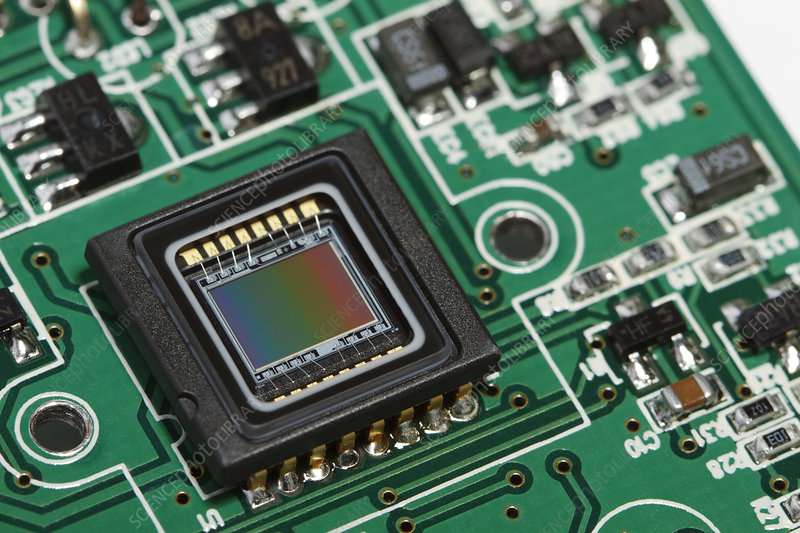
\includegraphics[height=0.27\textwidth]{Figures/CCD.jpg}
}
  \caption{Photorécepteurs usuels, avec leurs temps de réponse $\tau_r$.}
  \label{fig:photorec}
\end{figure}


\section{Émission de la lumière : sources lumineuses}

Nous nous sommes intéressés à la propagation de la lumière dans le cadre du modèle scalaire, mais pas encore à son émission ou son absorption. Dans cette section, nous étudions les sources lumineuses.

%Toutes les sources ne sont pas équivalentes pour observer des interférences bien contrastées, en particulier nous allons expliquer comment la polychromaticité de la source affecte la figure d'interférences.


\subsection{Processus physiques d’émission}
\label{sec:processus_emission}
% Comment expliquer l'écart aussi important de longueur de cohérence temporelle entre le laser et une source de lumière blanche ? Ces différences proviennent des processus à l’origine de l’émission de lumière et des propriétés physiques du milieu émetteur.
Les propriétés des sources lumineuses dépendent des processus d’émission à l’origine de la lumière émise. On distingue deux types de processus d’émission. Nous étudierons ces processus plus en détails lorsque nous discuterons du laser.

\parag{Émission spontanée}
  On appelle \imp{émission spontanée} le processus au cours duquel un atome excité, d'énergie élevée $E_2$, transite vers un état de plus basse énergie $E_1$ en émettant une vibration lumineuse de fréquence $\nu_{\rm m}$, voir \Fig{emission_spont}. La durée typique de cette émission est appelée \imp{durée de cohérence temporelle} et notée $\tau_{\rm{c}}$. La vibration lumineuse ainsi produite est appelée \imp{train d’onde}. La durée de cohérence temporelle pour l’émission spontanée vaut environ
  \eqbox[]{\tau_c \sim \SI{e-11}{s}.}

  \begin{definition}[Train d'onde]\label{def:}
    Un \imp{train d’onde} est une vibration monochromatique de durée finie $\tau_c$ émise par un atome excité. 
    %  lors d'une transition énergétique. Il est caractérisé par sa fréquence $\nu$, sa durée $\tau_c$, sa direction, sa polarisation, et sa phase.
  \end{definition}

  Chaque train d’onde a une direction, une polarisation, et une phase \imp{aléatoires} : les trains d'ondes émis par émission spontanée sont dits \imp{incohérents} entre eux, voir \Fig{train_spont}. La phase $\varphi_S$ de la vibration lumineuse émise par une source $S$ reste à peu près constante sur une durée $\tau_c$ ; puis l’émission est stoppée et reprend avec une phase $\varphi_S$ différente et aléatoire.

\begin{figure}[H]
  \centering
  \subfigure[]{\label{fig:emission_spont}
  
\includegraphics[scale=1]{emis_spont}
  }\hspace{1cm}
  \subfigure[]{\label{fig:train_spont}
  
\includegraphics[scale=1]{trains_spont}
  }
  \caption{(a) Schématisation du processus d'émission spontanée d'un train d’onde pour un atome à deux niveaux. Un atome émet spontanément une vibration lumineuse de fréquence $\nu$ et de durée typique $\tau_c$. (b) Les trains d’onde émis par émission spontanée sont de direction, de polarisation et de phase aléatoires.}
  \label{fig:}
\end{figure}


\parag{Émission stimulée}

Il existe aussi un autre processus d'émission induit par l’interaction de l'atome excité avec une vibration lumineuse. On appelle \imp{émission stimulée}, ou induite, le processus au cours duquel un atome excité, d'énergie élevée $E_2$, transite vers un état d’énergie plus basse $E_1$, sous l'effet de l’interaction avec un train d’onde de fréquence $\nu_{\rm m}$ et de durée typique $\tau_c$. L'atome réémet alors \imp{deux} trains d’onde \imp{cohérents} de fréquence $\nu_{\rm m}$ et de durée $\tau_c$. Ce phénomène est à la base de la physique du laser (\textit{Light Amplification by Stimulated Emission of Radiation}).  La durée de cohérence temporelle est plus longue pour l’émission stimulée que pour l’émission spontanée, et vaut environ
\eqbox[]{\tau_c \sim \SI{e-9}{s}.}

\begin{figure}[H]
\centering

\includegraphics[scale=1]{emis_sti}
\caption{Schématisation du processus d'émission stimulée pour un atome à deux niveaux. Un train d’onde incident de fréquence $\nu$ et de durée typique $\tau_c$ induit une désexcitation par l'émission d'un second train d’onde aux propriétés identiques au train d’onde incident. Les trains d’onde émis par émission stimulées ont donc même direction, même polarisation, et même phase.}
\label{fig:emission_stim}
\end{figure}

\subsection{Spectre d'émission}

\parag{Densité spectrale en fréquence}
 Considérons une source lumineuse dont le processus d’émission produit des trains d’onde de fréquence $\nu_{\rm m}$ et de durée $\tau_c$. L’analyse de Fourier nous enseigne qu’un signal de durée finie $\tau_c$ présente un élargissement en fréquence  $\Delta\nu$ dans son spectre, donné par la relation
% \begin{equation}
\eqbox{
  \Delta\nu \simeq \frac{1}{\tau_c}.
}
% \end{equation}
% En optique, cette durée $\tau_c$ s’interprète comme la \imp{durée de cohérence  temporelle} de la vibration lumineuse. Cette durée  est fixée par le temps caractéristique du processus d'émission (Sec.~\ref{sec:processus_emission}) et dépend donc du type de source.

Nous avons raisonné jusqu'à présent sur le modèle d’une lumière \emph{monochromatique}, de fréquence $\nu_{\rm m}$ bien définie.
 Nous voyons qu’en réalité, toute source de lumière est \emph{polychromatique} : elle émet dans un certain intervalle de fréquence, plus ou moins étroit, de largeur $\Delta \nu$.
Une source lumineuse est donc caractérisée par sa \important{densité spectrale en fréquence} $D(\nu)$, en $\SI{}{W.m^{-2}.Hz^{-1}}$, telle qu'une bande infiniment petite de largeur $\d \nu$ autour d'une fréquence $\nu$ contienne une intensité lumineuse $D(\nu)\,\d\nu$. 
L’intensité lumineuse totale émise $I$ s'obtient alors par intégration,
\begin{equation}
I=\int_{0}^{\infty}D(\nu)\,\d\nu.
\end{equation}
Dans le cas où le processus d’émission provient d’atomes indépendants à deux niveaux, la densité spectrale est piquée autour de $\nu_{\rm m}$ et de largeur typique $\Delta \nu$, comme sur la \Fig{Dnu}.
%%%%%%%%%%%%%%%%%%%%%
\begin{figure}[h!]
\centering
\subfigure[]{\label{fig:Dnu}

\includegraphics[scale=1.1]{Dnu}
}\hspace{1cm}
\subfigure[]{\label{fig:Dlambda}

\includegraphics[scale=1.1]{Dlambda}
}
\caption{(a) Allure de la densité spectrale en fréquence $D(\nu)$ en fonction de la fréquence $\nu$ pour une lumière émise par des atomes indépendants à deux niveaux d’énergie. Le spectre prend la forme d’une raie centrée en $\nu_0$ de largeur $\Delta \nu$. (b) Idem pour la densité spectrale en longueur d’onde $\tilde{D}(\lambda)$.}
\end{figure}
%%%%%%%%%%%%%

% La densité spectrale a typiquement l’allure présentée sur la \Fig{D} : un ou plusieurs pics de largeur typique $\Delta \nu$.

\parag{Densité spectrale en longueur d’onde} Le même raisonnement s’applique en longueur d’onde. Considérons une source lumineuse dont le processus d’émission produit des trains d’onde de longueur d’onde $\lambda_{\rm m}$ et de longueur $\ell_c = c\tau_c$, appelée \imp{longueur de cohérence temporelle}. Un écart en fréquence $\Delta \nu$ avec $\lambda = \frac{c}{\nu}$ correspond à un écart en longueur d’onde $\Delta \lambda = \Delta \nu \frac{c}{\nu^2} \simeq \frac{1}{\tau_c} \frac{c}{\nu^2} = \frac{c^2}{\nu^2}\frac{1}{\lc} = \frac{\lambda^2}{\lc}$, soit 
\eqbox{
\Delta \lambda \simeq \frac{\lambda_{\rm m}^2}{\lc}.
}

Une source lumineuse est caractérisée par sa \important{densité spectrale en longueur d’onde} $\tilde{D}(\lambda)$, exprimée en $\SI{}{W.m^{-2}.nm^{-1}}$, telle qu’une bande infiniment petite de largeur $\d \lambda$ autour d’une longueur d’onde $\lambda$ contienne une intensité lumineuse $\tilde{D}(\lambda)\,\d\lambda$. L’intensité lumineuse totale émise $I$ s'obtient alors par intégration,
\begin{equation}
I=\int_{0}^{\infty}\tilde{D}(\lambda)\,\d\lambda.
\end{equation}
Dans le cas où le processus d’émission provient d’atomes indépendants à deux niveaux, la densité spectrale est piquée autour de $\lambda_{\rm m}$ et de largeur typique $\Delta \lambda$, comme sur la \Fig{Dlambda}.

\begin{exemple}{Densité spectrale en longueur d’onde}
  Exprimer $\tilde{D}(\lambda)$ en fonction de $D(\nu)$ en s'aidant du changement de variable $\lambda = \frac{c}{\nu}$.
\end{exemple}
\examplesol{
La densité spectrale en longueur d’onde est définie par
$$
I=\int_{0}^{\infty}D(\nu)\,\d\nu=\int_{0}^{\infty}\tilde{D}(\lambda)\,\d\lambda.
$$
En effectuant le changement de variable $\nu=c/\lambda$, la mesure est transformée en $\d\nu = -c/\lambda^2\,\d\lambda$, et on obtient
$$
I = \int_{0}^{\infty}D(\nu)\,\d\nu =  \int_{\infty}^{0}\frac{c{D}(\nu)}{\lambda^2}\,\d\lambda,
$$
d'où l'on tire 
\eqbox{
\tilde{D}(\lambda) = D\left( \nu=\frac{c}{\lambda} \right)\frac{c}{\lambda^2}.
}

% On obtient aussi la largeur en longueur d’onde $\Delta \lambda$, assimilé à un infiniment petit, en écrivant que
% $$
% \frac{\Delta \lambda}{\Delta \nu} \simeq \norm{\frac{\d \lambda}{\d \nu}(\nu=\nu_0)} = \frac{c}{\nu_0^2}= \frac{\lambda0^2}{c}  \Rar \Delta \lambda \simeq \Delta \nu \frac{\lambda_0^2}{c}.
% $$
}

%  Les trains d’onde se propagent à la vitesse $c$ : un train d’onde de durée $\tau_c$ a donc une longueur $\ell_c = c \tau_c$, appelée \imp{longueur de cohérence temporelle}. L’analyse de Fourier permet de même d’exprimer $\ell_c$ en fonction de la largeur en longueur d’onde $\Delta \lambda$.

%  \begin{exemple}{Longueur de cohérence temporelle}
% À partir de la relation entre $\tau_c$ et $\Delta \nu$, relier $\ell_c$ à $\Delta \lambda$.
%  \end{exemple}
%  \examplesol{
%  Il suffit d’écrire que
%  $$
% \ell_c = c \tau_c \sim \frac{c}{\Delta \nu} \simeq \frac{\lambda_0^2}{\Delta \lambda}.
%  $$
%  }

\begin{prop}[Propriété spectrale d'une source lumineuse]
Un source lumineuse qui émet des trains d’onde de 
$
\left\{
\begin{array}{l}
  \text{durée } \tau_c, \\ 
  \text{longueur } \lc = c \tau_c, \\
\end{array}
\right.
$\\
présente un spectre lumineux de 
$
\left\{
\begin{array}{l}
  \text{largeur en fréquence } \Delta \nu \simeq \displaystyle\frac{1}{\tau_c}, \\[0.3cm] 
  \text{largeur en longueur d’onde } \Delta \lambda \simeq \displaystyle\frac{\lambda_{\rm m}^2}{\lc}.
\end{array}
\right.
$
\end{prop}

\begin{figure}[H]
  \centering
  \subfigure[]{
  
\includegraphics[height=0.28\textwidth]{laser2}
  }
  \subfigure[]{
  
\includegraphics[height=0.28\textwidth]{lampe_spectrale2}
  }
  \subfigure[]{
  
\includegraphics[height=0.28\textwidth]{QI}
  }
  \caption{(a) Diode laser verte. (b) Lampe spectrale basse pression. \Wiki.~(c) Lampe halogène similaire aux lampes quartz-iode de TP. \Wiki}
\end{figure}

\parag{Exemples de sources lumineuses} Vous devez être capable de classer les sources suivantes en fonction de leur durée et longueur de cohérence. Il est également préférable de connaître les mécanismes physiques à l’œuvre et l’allure du spectre. Les trois sources principales sont les suivantes.
\begin{liste}
\item \udl{Laser}.
Un laser fonctionne sur le principe de l’émission stimulé : il émet donc une raie quasi monochromatique dont les trains d'onde sont de durée $\tau_c \sim \SI{1}{ns}$, soit une largeur spectrale en fréquence $\Delta \nu \sim \SI{1}{GHz}$.

\begin{remarque}
  Un laser contient un milieu amplificateur et une une cavité résonnante qui sélectionne une seule raie (laser monomode) ou un petit nombre de raies (laser multimode). Les lasers monomodes utilisés en recherche ont une largeur spectrale exceptionnelle de $\Delta \nu \sim \SI{100}{kHz}$.
\end{remarque}

\item \udl{Lampe spectrale}.
Une lampe spectrale contient une vapeur atomique excitée par un arc électrique.  Les lampes spectrales les plus connues sont celles au sodium $\rm Na$ et au mercure $\rm Hg$. Dans une lampe à basse pression, les atomes sont quasi isolés, et possèdent donc plusieurs niveaux d’énergie proches de ceux déterminés par la théorie de Bohr de l’atome d’hydrogène. Les atomes émettent suivant le principe de l'émission spontanée, dont les trains d'onde sont de durée $\tau_c \sim \SI{10}{ps}$, ce qui conduit à un spectre de raies fines, de largeur spectrale intrinsèque $\Delta \nu \sim \SI{100}{GHz}$ en fréquence.


\begin{remarque}
  Dans les lampes spectrales haute pression, utilisées dans l'éclairage public, les raies spectrales sont élargies par effet Doppler et par collision entre les atomes. La largeur spectrale est alors beaucoup plus élevée, typiquement $\Delta \nu \sim \SI{1}{THz}$.
\end{remarque}


\item \udl{Lumière blanche}.
Une source de lumière blanche (comme le Soleil ou une lampe quartz-iode) est une source thermique :  la lumière contient toutes les couleurs et apparaît donc blanche. La durée d'un train d'onde vaut $\tau_c \sim \SI{3}{fs}$, soit une largeur spectrale en fréquence $\Delta \nu \sim \SI{300}{THz}$, du même ordre de grandeur que la fréquence émise. 
\begin{remarque}
  
  La lumière solaire est centrée sur $\lambda\simeq\SI{600}{nm}$ pour une largeur en longueur d’onde $\Delta\lambda\simeq\SI{300}{nm}$ ($\Delta \nu = \SI{300}{THz}$ en fréquence), d'où une longueur de cohérence $l_{\rm{c}}\sim \SI{1}{\mu\meter}$ (durée de cohérence $\tau_c \sim \SI{3}{fs}$).
  % \footnote{En sortie d’un filtre interférentiel, de largeur spectrale $\Delta \lambda \simeq \SI{20}{nm}$, la cohérence temporelle  vaut $\lc \sim \SI{30}{\mu m}$.}.
\end{remarque}
  \begin{remarque}
    Une source thermique est une phase dense, dont les niveaux énergétiques des atomes sont modifiés par l’interaction chimique avec les atomes environnants, ce qui conduit à une bande continue d’énergie. Les atomes n’émettent donc pas de raie, mais un spectre continu qui obéit plus ou moins à la loi de Planck du corps noir. La largeur spectrale en fréquence vaut typiquement $\Delta \nu \simeq \frac{\kB T}{h}$, et croit avec la température.
\end{remarque}
\end{liste}

\begin{exemple}{Longueur de cohérence et largeurs spectrales de sources usuels}
  À partir des durées de train d'onde $\tau_c$ données précédemment, déterminer la longueur de cohérence $\lc$ et la largeur spectrale en longueur d'onde $\Delta \lambda$ pour les trois sources lumineuses du tableau ci-dessous.
    \begin{center}
      \begin{tabular}{|c|c|c|c|}
        \hline
        Source & \textsc{laser} & \textsc{lampe spectrale} & \textsc{lumière blanche} \\
        \hline
        Exemple & diode laser rouge & lampe Na basse pression & lampe quartz-iode \\
        \hline
        $\lambda_{\rm m}$ & $\SI{631}{nm}$ & $\SI{589}{nm}$ &  $\SI{600}{nm}$\\
        \hline
        $\lc$ &  &  &  \\
        \hline
        $\Delta \lambda$ &  &  & \\
        \hline
      \end{tabular}
    \end{center}
\end{exemple}
\examplesol{
    \begin{center}
      \begin{tabular}{|c|c|c|c|}
      \hline
      Source & \textsc{laser} & \textsc{lampe spectrale} & \textsc{lumière blanche} \\
      \hline
      Exemple & diode laser rouge & lampe Na basse pression & lampe quartz-iode \\
      \hline
      $\lambda_{\rm m}$ & $\SI{631}{nm}$ & $\SI{589}{nm}$ &  $\SI{600}{nm}$\\
      \hline
      $\lc$ & $\SI{30}{cm}$ & $ \SI{3}{mm}$ & $\SI{1}{\micro\meter}$ \\
      \hline
      $\Delta \lambda$ & $\SI{1}{pm}$ & $ \SI{0.1}{nm}$ & $ \SI{300}{nm}$ \\
      \hline
    \end{tabular}
  \end{center}
}

\begin{experience}{Spectres de sources lumineuses usuelles}\label{exp:spectres}
  On peut déterminer le spectre d'une source avec spectromètre. Cet appareil utilise la dispersion du faisceau lumineux à travers un prisme pour séparer et identifier chaque composante du spectre. Le spectromètre de TP a une précision d'environ $\SI{1}{nm}$. Tracer l’allure du spectre expérimental pour chaque source : diode laser rouge, lampe spectrale basse pression à vapeur de sodium, ou lampe quartz-iode.
  
%   \begin{fig}[]
%     \centering
%     \begin{subfig}[label][0.45]
%       
\includegraphics[width=0.8\textwidth]{Sodium_Spectra}
%     \end{subfig}
% \begin{subfig}[label][0.45]
%   
\includegraphics[width=0.8\textwidth]{QI_spectre}
% \end{subfig}
%     \capt{Exemples de spectres lumineux.}
%   \end{fig}

\end{experience}

% \begin{table}[h!]
%   \centering
%   \begin{tabular}{|c|c|c|c|}
%     \hline
% Type de source & \textsc{laser} & \textsc{lampe spectrale} & \textsc{lumière blanche} \\
% \hline
% Exemple & diode laser rouge & lampe Na basse pression & lampe quartz-iode \\
% \hline
% $\lambda$ & $\SI{631}{nm}$ & $\SI{589}{nm}$ &  $\SI{600}{nm}$\\
% \hline
% $\Delta \lambda$ & $\SI{e-3}{nm}$ & $ \SI{e-1}{nm}$ & $ \SI{300}{nm}$ \\
% \hline
% $\lc$ & $\SI{30}{cm}$ & $ \SI{3}{mm}$ & $\SI{1}{\mu\meter}$ \\
% \hline
%   \end{tabular}
%   \caption{Propriétés spectrales des trois types de source lumineuse usuels.}
%   \label{}

% \end{table}
% \end{liste}
\begin{remarque}
On distingue également d’autres sources de lumière.
\begin{liste}
\item Les lampes à incandescence émettent un rayonnement qui dépend de la température d'un filament (en général en tungstène) chauffé lorsqu'il est traversé par un courant électrique (effet Joule). Ces lampes émettent en général dans l'infrarouge et par conséquent chauffent de façon importante.
\item Pour prolonger la durée de vie du filament, on rajoute des éléments halogènes dans l'ampoule sous forme de gaz à basse pression: ce sont les lampes halogènes que l'on tend à remplacer dans la vie courante par les DELs (diodes électroluminescentes). La lampe quartz-iode est un type particulier de lampe halogène.
\item  Les DELs présentent un fonctionnement différent car elles sont composées d'un semi-conducteur. Pour simplifier grossièrement, le semi-conducteur émet des photons possédant une énergie bien déterminée lorsqu'il est parcouru par un courant électrique: le spectre qui en résulte est donc discret\footnote{On rajoute parfois une couche fluorescente qui permet d'absorber une partie de la lumière et de réémettre dans une zone spectrale plus large. On observe alors une superposition des spectres discret de la DEL et continu de la substance fluorescente. Cette technique de couche fluorescente est aussi employée dans les lampes à décharge fluo-compactes (aussi appelées lampes basse consommation ou à économie d'énergie).}.
\end{liste}
\end{remarque}


\end{document}
